\documentclass[../main.tex]{subfiles}

\begin{document}
\begin{CJK*}{UTF8}{gbsn}

\section*{Exercice 1f}
On se demande si d'autres variables
dans le jeu de données pourraient être des facteurs confondants, et si l'on devrait stratifier le
test du Log-Rank sur l'une de ces variables. À partir de statistiques descriptives, de graphiques
et/ou d'arguments adaptés au contexte de l'étude, discuter de laquelle des variables du jeu de
données risque d'agir comme facteur confondant et reproduire le test du Log-Rank stratifié pour cette variable.
    
\paragraph{Solution}
Dans la vie quotidienne, on trouve que des personnes 
âgées ont plus grande probabilité de devenir aveugle. 
On soupçonne naturellement que l'âge
soit un facteur confondant qui influence la durée jusqu'à la cécité.
On utilise donc l'âge comme la variable à analyser. 
On va d'abord tracer les courbes de survie pour les deux groupes de l'âge.
Notamment, on classe les patients en deux groupes, "Younger" et "Older",
selon si l'âge du patient soit inférieur ou supérieur à l'âge médian.
Pour ce faire, on commence par la graphique Kaplan-Meier pour les deux groupes,
en utilisant le rouge pour représenter le groupe "Younger" 
et le bleu pour représenter le groupe "Older". 
Le graphique montre que la courbe rouge est plus élevée que la courbe bleue 
à la plupart des moments, ce qui signifie que la probabilité de survie est plus 
élevée pour le groupe "Younger" que pour le groupe "Older". 

\begin{lstlisting}
    median_age <- median(diabetic$age, na.rm = TRUE)
    diabetic$age_group <- ifelse(diabetic$age <= median_age, "younger", "older")
    result.kmage <- survfit(Surv(time, status) ~ age_group, data = diabetic)
    plot(result.kmage, main = 'Courbe de Kaplan-Meier', xlab = 'Temps en jours', ylab = 'Probabilite de survie', col = c("red", "blue"))
\end{lstlisting}

Le plot est :

\begin{figure}[H]
    \centering
    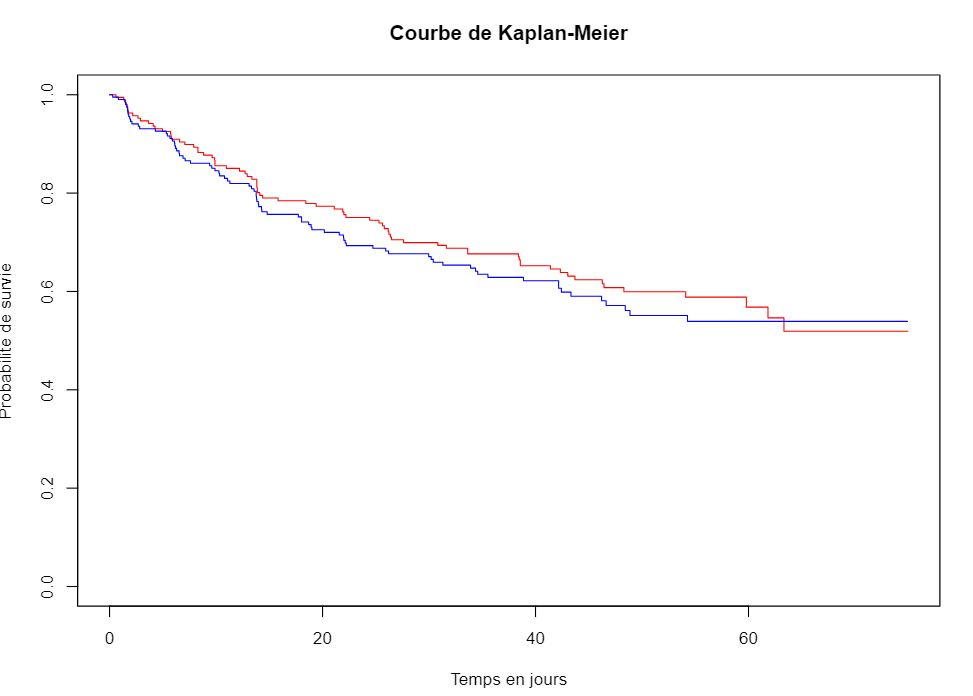
\includegraphics[width=0.8\textwidth]{1F.JPG}
    \label{fig:mesh1}
\end{figure}
  
Sur cette graphique on peut trouver que le groupe de patients "Younger"
présente une probabilité de cécité plus faible que le groupe de patients "Older".
Par conséquent, on conclut que l'âge est un facteur important.
On effectue le test de Log-Rank stratifié pour les deux groupes d'âge.

\begin{lstlisting}
    survdiff(Surv(time, status) ~ trt + strata(age), data = diabetic)
\end{lstlisting}

Le résultat est :

\begin{lstlisting}    
Call:
survdiff(formula = Surv(time, status) ~ trt + strata(age), data = diabetic)
        
        N Observed Expected (O-E)^2/E (O-E)^2/V
trt=0 197      101     71.9      11.8      23.4
trt=1 197       54     83.1      10.2      23.4
        
    Chisq= 23.4  on 1 degrees of freedom, p= 1e-06
\end{lstlisting}

Comme la p-valeur est $1e-06$,
il y a une différence significative dans le délai de cécité entre les deux groupes de traitement.
Même après stratification par âge, il existe toujours une différence 
significative dans le risque de cécité entre le groupe \texttt{trt=1}
et le groupe de \texttt{trt=0}. 
On conclut que les patients du groupe de \texttt{trt=1} ont une probabilité de cécité plus faible que 
les patients du groupe \texttt{trt=0}. 
En conclusion, l'âge est un facteur important influençant la durée 
de la cécité et qu'il doit être pris en compte lors de l'élaboration des stratégies de traitement. ////

\end{CJK*}
\end{document}